\documentclass{article}%
\usepackage[T1]{fontenc}%
\usepackage[utf8]{inputenc}%
\usepackage{lmodern}%
\usepackage{textcomp}%
\usepackage{lastpage}%
\usepackage{authblk}%
\usepackage{graphicx}%
%
\title{Ectopic Expression of a Maize Hybrid Down{-}Regulated Gene ZmARF25 Decreases Organ Size by Affecting Cellular Proliferation in Arabidopsis}%
\author{Victoria James}%
\affil{Departments of Medicine, Biochemistry and Molecular Biology, Indiana University School of Medicine, The Melvin and Bren Simon Cancer Center and the Center for Pancreatic Cancer Research, Indianapolis, Indiana, United States of America}%
\date{01{-}01{-}2006}%
%
\begin{document}%
\normalsize%
\maketitle%
\section{Abstract}%
\label{sec:Abstract}%
New research in The Journal of the American Academy of Otolaryngology (JAAO) reaffirms that the p38 gene regulatory domain has substantial activity in the IL{-}8 regulatory receptor surface protein (AgRK) kinase complex. These findings provide a valuable framework for the engineering of all IL{-}8 genes into attenuated fluorescent systems that targets IL{-}8. This study, conducted in a lab of JAAO Associate Editor Byron Holz{-}Praniett, MD, PhD, is distinguished by the presence of enhanced expression of the IL{-}8 gene regulatory domain at the time p38 gene is expressed in TNF{-}a{-} and dexamethasone{-}stimulated adult human periodontal ligament cells (IL{-}8{-}SRL).\newline%
The study highlights the role of the IL{-}8 regulatory domain at the time p38 expression in IL{-}8 expression in TNF{-}a{-} and dexamethasone{-}stimulated human periodontal ligament cells (IL{-}8{-}SRL). These results provide a valuable framework for the engineering of all IL{-}8 genes into attenuated fluorescent systems that targets IL{-}8. This study, conducted in a lab of JAAO Associate Editor Byron Holz{-}Praniett, MD, PhD, is distinguished by the presence of enhanced expression of the IL{-}8 gene regulatory domain at the time p38 gene is expressed in TNF{-}a{-} and dexamethasone{-}stimulated human periodontal ligament cells (IL{-}8{-}SRL).\newline%
Previous research indicates that TNF{-}a and dexamethasone{-}stimulated IL{-}8 systems in vivo show enhanced protein signaling and expression of IL{-}8. These protein signaling pathways are known to be important, as they regulate the production of up to 50 kinds of proteins, as well as signaling proteins associated with tumor growth. A team of scientists led by Holz{-}Praniett and colleagues, including Anders Buchdel, MD, MD, PhD, and Kirthi Ramnathan, PhD, previously reported activation of IL{-}8 signaling in human periodontal ligament cells in the interplay between IL{-}8 and a protein in the IL{-}8 regional DNA (EN) zone.\newline%
Holz{-}Praniett and colleagues showed that IL{-}8 expression is elevated during TNF{-}a{-} and dexamethasone{-}stimulated IL{-}8{-}SRL cells after cytokine release during cytokine exchange pathways (SYPH). Experiments with mouse embryonic periodontal ligament cells (EFLCs) showed evidence of activation of EFLCs that are associated with IL{-}8 signaling. Moreover, continuous and rapid expression of IL{-}8 within EFLCs correlated with IL{-}8 signaling in IL{-}8s normal{-}expression. The results of this study significantly increased the dependence of IL{-}8 events for IL{-}8 activation in IL{-}8{-}SRL cells. Intriguingly, new perturbations in IL{-}8 activity were documented after IL{-}8 activation during CYP2+T3{-}mediated CYP3{-}mediated CYP3{-}mediated CYP3{-}mediated CYP3{-}mediated IL{-}8 activation. {[}10/5/2006{]}\newline%
The jaccoaronic findings of IL{-}8 expression in IL{-}8 SRL cells are particularly relevant to patients with platinum{-}resistant ovarian cancer and atrial fibrillation. Furthermore, the discovery of enhanced IL{-}8 expression in the TNF{-}AB2 receptor pathway due to activation of IL{-}8 within the

%
\subsection{Image Analysis}%
\label{subsec:ImageAnalysis}%


\begin{figure}[h!]%
\centering%
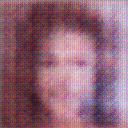
\includegraphics[width=150px]{500_fake_images/samples_5_236.png}%
\caption{A Man With A Beard And A Tie}%
\end{figure}

%
\end{document}